\documentclass[a4paper]{article}

\usepackage[english]{babel}
\usepackage[utf8]{inputenc}
\usepackage{csquotes}
\usepackage{amsmath, latexsym}
\usepackage{graphicx}
\usepackage{tikz}
\usepackage{listings}
\usepackage{verbatim}
\usepackage{bigints}
\usepackage{float}
\usepackage{titling}
\usepackage[colorinlistoftodos]{todonotes}
\usepackage[style=authoryear,sorting=nty,maxcitenames=1]{biblatex}



\title{Computation of far-field acoustic waves emitted by axisymmetric bubble collapse}
\author{}
\date{\today}
\addbibresource{references.bib}



\begin{document}
\maketitle
\section{Mathematical formulation}
\begin{figure}[h!]\label{schematic}
	\centering
	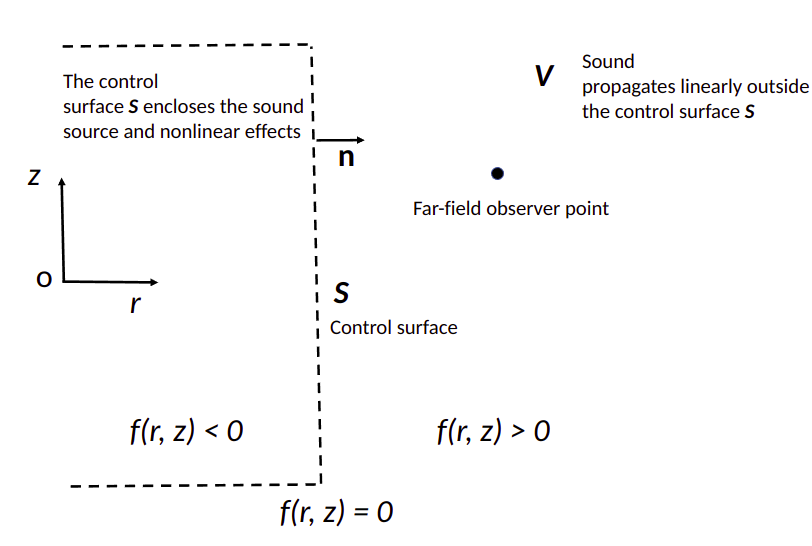
\includegraphics[width=12cm]{images/shematic.png}
	\caption{Stationary control surface $S$ encloses sound source}
\end{figure}
In this section, we derive the Kirchhoff formula for an axisymmetric problem. We chose a control surface $S$ such that it encloses all the acoustic sources, and the sound propagates linearly outside the control surface. Therefore, the pressure perturbation $p$ satisfies the homogeneous wave equation in the region $V$ (\ref{schematic}).  Assuming axisymmetry, the acoustic wave equation in the cylindrical coordinate system is given by 
\begin{equation}\label{Wave equation}
	\Bigg( \frac{1}{c_{0}^2}\frac{\partial{}^{2}}{\partial{t}^{2}}- \frac{\partial^2}{\partial r^2} - \frac{1}{r}\frac{\partial}{\partial r} - \frac{\partial^2}{\partial z^2}\Bigg) p = 0 \quad \quad \textrm{in} \ V.
\end{equation}
The control surface S is defined by $f(r, z) = 0$, $f(r, z) > 0$ for $r, z$ in V and $f(r, z) < 0$ for $r, z$ inside surface S. Then the Heaviside function of $f(r, z)$ is
\begin{equation}\label{Heaviside}
	H(f) =\begin{cases}
		1, & \text{for $r, z$ in V}.     \\
		0, & \text{for $r, z$ inside S}.
	\end{cases}
\end{equation}
We define the perturbation pressure $p$ as a generalized function $pH(f)$ (\cite{ffowcs1969sound}) where
\begin{equation}\label{Generalized_Functions}
	p H(f) =\begin{cases}
		p , & \text{for $r, z$ in V}.     \\
		0,  & \text{for $r, z$ inside S}.
	\end{cases}
\end{equation}
The generalized pressure $pH(f)$ is defined everywhere in space, unlike $p$ defined only in $V$. We will derive the acoustic wave equation for the generalised pressure. The partial derivative of generalized pressure in space and time is
\begin{equation}\label{r derivative}
	\frac{1}{r}\frac{\partial }{\partial r}(pH) = \frac{1}{r}\frac{\partial p}{\partial r}H + \frac{1}{r}p\delta(f)\frac{\partial f}{\partial r},
\end{equation}
\begin{equation}\label{rr derivative}
	\frac{\partial^2}{\partial r^2}(pH) = \frac{\partial^2 p}{\partial r^2}H + \frac{\partial p}{\partial r}\delta(f)\frac{\partial f}{\partial r} + \frac{\partial}{\partial r}(p\delta(f)\frac{\partial f}{\partial r}),
\end{equation}
\begin{equation}\label{z derivative}
	\frac{\partial^2}{\partial z^2}(pH) = \frac{\partial^2 p}{\partial z^2}H + \frac{\partial p}{\partial z}\delta(f)\frac{\partial f}{\partial z} + \frac{\partial}{\partial z}(p\delta(f)\frac{\partial f}{\partial z}),
\end{equation}
and
\begin{equation}\label{Time derivative}
	\frac{\partial^2}{\partial t^2}(pH) = \frac{\partial^2 p }{\partial t^2}H.
\end{equation}
We premultiply (\ref{Time derivative}) with $1/{c_{0}^2}$ and subtract (\ref{r derivative}, \ref{rr derivative}, \ref{z derivative}) to obtain the inhomogeneous acoustic wave equation in generalised pressure
\begin{equation}\label{Generalized wave equation}
	\Bigg( \frac{1}{c_{0}^2}\frac{\partial{}^{2}}{\partial{t}^{2}}- \frac{\partial^2}{\partial r^2} - \frac{1}{r}\frac{\partial}{\partial r} - \frac{\partial^2}{\partial z^2}\Bigg) pH = s(r, z, t).
\end{equation}
where
\begin{equation}\label{Source}
	\begin{split}
		s(r, z, t) =& -\frac{1}{r}p\delta(f)\frac{\partial f}{\partial r}
	-\frac{\partial p}{\partial r}\delta(f)\frac{\partial f}{\partial r}
	-\frac{\partial p}{\partial z}\delta(f)\frac{\partial f}{\partial z}
	-\frac{\partial}{\partial r}(p\delta(f)\frac{\partial f}{\partial r})\\
	&-\frac{\partial}{\partial z}(p\delta(f)\frac{\partial f}{\partial z})
	\end{split}.
\end{equation}
The source term is non-zero only at surface $S$, as it contains $\delta (f)$. The acoustic wave equation (\ref{Generalized wave equation}) in generalized variables is valid in the entire unbounded space. Therefore we can use the free-space Green's function to solve the equation. The Green's function is the solution of wave equation for an impulsive point source $\delta(r - r')\delta(z - z')\delta(t - \tau)$ placed at point $r', z'$ and time $\tau$
\begin{equation}\label{green}
	\Bigg( \frac{1}{c_{0}^2}\frac{\partial{}^{2}}{\partial{t}^{2}}- \frac{\partial^2}{\partial r^2} - \frac{1}{r}\frac{\partial}{\partial r} - \frac{\partial^2}{\partial z^2}\Bigg) {G(r, z, t; r', z', \tau )} = \delta(r - r')\delta(z - z')\delta(t - \tau).
\end{equation}
Once the Green's function is obtained the solution of the inhomogeneous acoustic wave equation \ref{Generalized wave equation} is 
\begin{equation}\label{pressure}
	pH(r, z, t) = \int_{\tau}\int_{z'}\int_{r'} s(r', z', \tau)G(r, z, t; r', z', \tau ) dr'dz'd\tau.
\end{equation}
\printbibliography
\end{document}


